\begin{enumerate}[label =]
    \item \textbf{($\Rightarrow$)}
    Suppose for any finite diagram limit exists.
            \begin{enumerate}[label=(\textit{\roman*})]
                \item 
                    let $\mathcal I_0 = \{\}$.
                    since $X = \lim_{\leftarrow \mathcal I_0} \mathcal D_0$
                    exists, and the image of $\mathcal I$ in $\mathcal C$ is empty,
                    therefore any object of $\mathcal C$ like $Y$ with any morphisms, commutes with this emtpy Image of $\mathcal I$. Which means that there exists a unique morphism $Y \xrightarrow{\varphi} X$.
                    Therefore we can say that there exists a unique morphism from any object of $\mathcal C$ to $X$. This shows that $X$ is terminal object of the cateogry $\mathcal C$.
                \item 
                    Let $A, B \in \mathcal C_0$. Let $\mathcal I$ be the category of 2 with only identity morphisms.
                    \begin{center}
                        
                        \tikz{
                            \node at (-1, 0) (A) {.};
                            \node at (1, 0) (B) {*};

                            \path[->]          
                                (A) edge [loop above] node {id} (A)
                                (B) edge [loop above] node {id} (B);
                            }   
                    \end{center}
                    Where $\mathcal D$ maps $.$ to $A$ and $*$ to $B$. Let $X = \lim_{\leftarrow \mathcal{I}} \mathcal D$ with morphisms $P_A$ and $P_B$ be the limit of this diagram.
                    Now for any $f$ and $g$ we know that there exists a unique morphism $\varphi$ from $Y$ to $X$ such that the diagram commutes.
                    \begin{center}

                        \tikz{
                            \node at (-4, 0) (A) {$A$};
                            \node at (4, 0) (B) {$B$};
                            \node at (0, 1) (X) {$X = \lim_{\leftarrow \mathcal I} \mathcal D$};
                            \node at (0, 4) (Y) {$Y$};
                            \node at (-1, 2) (1) {$=$};
                            \node at (1, 2) (2) {$=$};

                            \path[->]
                                (A) edge [loop below] node {id} (A)
                                (X) edge [above] node {$P_A$} (A)
                                (X) edge [above] node {$P_B$} (B)
                                (Y) edge [above] node {$f$}   (A)
                                (Y) edge [above] node {$g$}   (B)
                                (Y) edge [right] node {$\exists ! \varphi$} (X)
                                (B) edge [loop below] node {id} (B);
                        }
                    \end{center}
                    Since for any $f$ and $g$, $Y$ commutes with the image of $\mathcal I$, therefore we can say that for any $f$ and $g$ there exists a unique morphism from $Y$ to $X$ such that the diagram above commutes.
                    With this description $X$ is the product of $A$ and $B$.    
                \item 
                    As for equalizer of two morphisms $f$ and $g$ from $A$ to $B$, let $\mathcal I$ be the cateogry of 2 with 2 non-trivial morphisms.
                    \begin{center}
                        \tikz{
                            \node at (-1, 0) (A) {$.$};
                            \node at (1, 0) (B) {$*$};

                            \path[->]
                                (A) edge [bend right] (B)
                                (A) edge [bend left] (B);
                        }
                    \end{center}
                    And let functor $\mathcal D$ be in a way that maps $.$ to $A$ and $*$ to $B$ and two non-trivial morphisms to $f$ and $g$.
                    Let $X = \lim_{\leftarrow \mathcal I} \mathcal D$ and morphisms $P_A$ and $P_B$ be the limit of this diagram $\mathcal D$.
                    \begin{center}
                        \tikz{
                            \node at (-4, 0) (A) {$A$};
                            \node at (4, 0) (B) {$B$};
                            \node at (0, 0) (1) {$=$};
                            \node at (1, 2) (2) {$=$};
                            \node at (-1, 2) (3) {$=$};
                            \node at (0, 1) (X) {$X = \lim_{\leftarrow \mathcal I} \mathcal D$};
                            \node at (0, 4) (Y) {$Y$};

                            \path[->]
                                (X) edge [above] node {$P_B$} (B)
                                (Y) edge [above] node {$\sigma$} (A)
                                (Y) edge [above] node {$\delta$} (B)
                                (Y) edge [right] node {$\exists ! \varphi$} (X)
                                (A) edge [bend right=25, above] node {$f$} (B)
                                (A) edge [bend right=35, below] node {$g$} (B)
                                (X) edge [above] node {$P_A$} (A);

                        }
                    \end{center}
                    Since $X$ commutes with image of $\mathcal I$ we have $fP_A = gP_A = P_B$.
                    Now let $Y$ be in a way such that it commutes with Image of $\mathcal I$. Then we have: $f \sigma = g\sigma = \delta$.
                    Now since $X$ is the limit of this diagram we know that there exists a unique $\varphi$ from $Y$ to $X$ such that it commutes.
                    This shows that $(X, P_A)$ is exactly the equalizer of $f$ and $g$. Since we have $fP_A = gP_A$. And also for any other $Y$ and $\sigma$ such that $f\sigma = g\sigma$ there exists a unique morphism from $Y$ to $X$ such that $\sigma = P_A \varphi$.
                    
                \end{enumerate}
    \item ($\Leftarrow$)
            Now suppose we have all 3 properties in $\mathcal C$. We want to prove that for any arbitrary finite index category $\mathcal I$ and diagram $\mathcal D$ there exists a limit.
            Let all of the objects in image of $\mathcal I$ be $D_1, D_2, \dots, D_n$.
            Since product of any number of objects is available in $\mathcal C$ consider $X = \Pi_{i = 1}^{n} D_i$.
            With morphisms $\pi_i$. But this diagram doesn't necessarily commute.
            For any $(Z, f_1, \dots, f_n)$ where $Z \overset{f_i }{\to } D_i$, that commutes with image of $\mathcal I$ there exists a unique morphism from $Z$ to $X$ such that the diagram commutes.
            \begin{equation}
                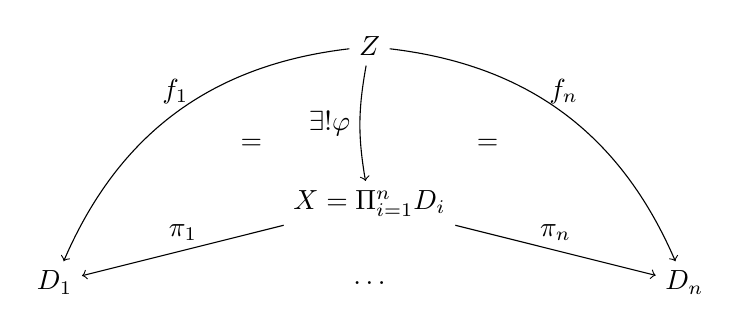
\begin{tikzpicture}
                    \node at (-4, 0) (D_1) {$D_1$};
                    \node at (4, 0) (D_n) {$D_n$};
                    \node at (0, 1) (X) {$X = \Pi_{i = 1}^{n} D_i$};
                    \node at (0, 3) (Z) {$Z$};
                    \node at (0, 0) (dots) {$\dots$};
                    \node at (1.5, 1.75) (=) {$=$};
                    \node at (-1.5, 1.75) (=) {$=$};
                    
                    \path[->]
                        (Z) edge [bend right, above] node {$f_1$} (D_1)
                        (Z) edge [bend left, above] node {$f_n$} (D_n)
                        
                        
                        (X) edge [above] node {$\pi_n$} (D_n)
                        (Z) edge [bend right=10,left] node {$\exists ! \varphi$} (X)
                        % (D_2) edge [bend left=10, below] node {$k$} (D_1)
                        (X) edge [above] node {$\pi_1$} (D_1);
                \end{tikzpicture}
            \end{equation}
            Now suppose object $Y$ with morphisms $\pi_1, \dots, \pi_n$ to $D_1, \dots, D_n$ where for the set $U$ of morphisms in image of $\mathcal I$ diagram commutes. in other words:
            \begin{gather*}
                \forall k \in U  \ \ s.t \ \  D_i \overset{k}{\to} D_j \\
                \implies \pi_j = k \pi_i
            \end{gather*}
            Also for any $(Z, f_1, \dots, f_n)$ that commutes with image of $\mathcal I$ then there exists a unique morphism $(\varphi)$ from $Z$ to $Y$ such that the diagram commutes or: $\forall i: f_i = \pi_i \varphi$. 
            Let $k$ be a morphism in image of $\mathcal I$ where $k: D_i \to D_j \notin U$. This means that $\pi_j \ne k \pi_i$. Now let $(Y', \sigma)$ be the equalizer of $\pi_j$ and $k \pi_i$. Therefore $\pi_j \sigma = k \pi_i \sigma$. We will show that $Y'$ has all the properties of $Y$ with a bigger $U$. \\
            Let $(Z, f_1, \dots, f_n)$ be in such a way that it commutes with image of $\mathcal I$. Then we know there exists a unique morphism from $Z$ to $Y$ such that the diagram commutes.
            \begin{equation}
                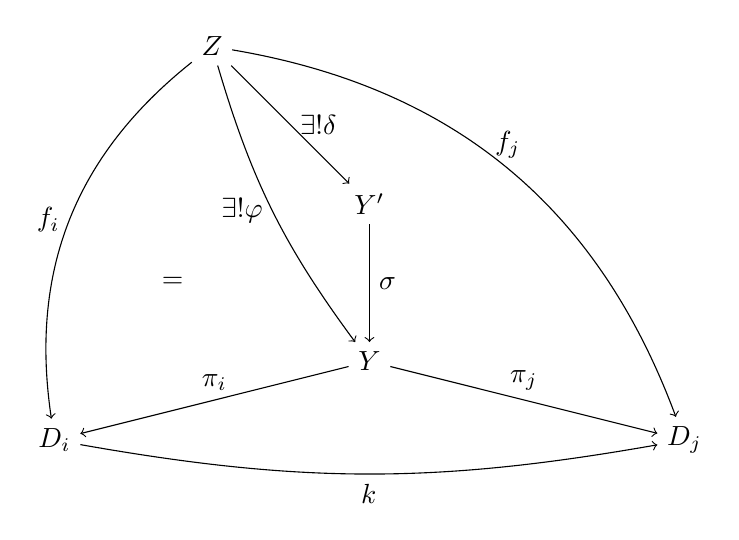
\begin{tikzpicture}
                    \node at (-4, 0) (D_i) {$D_i$};
                    \node at (4, 0) (D_j) {$D_j$};
                    \node at (0, 1) (Y) {$Y$};
                    \node at (0, 3) (Y1) {$Y'$};
                    \node at (-2, 5) (Z) {$Z$};
                    \node at (-2.5, 2) (=) {$=$};
                    
                    \path[->]
                        (Z) edge [bend right, left] node {$f_i$} (D_i)
                        (Z) edge [bend left, above] node {$f_j$} (D_j)
                        (Y1) edge [right] node {$\sigma$} (Y)
                        (D_i) edge [below, bend right=10] node {$k$} (D_j)
                        (Y) edge [above] node {$\pi_j$} (D_j)
                        (Z) edge [above, right] node {$\exists ! \delta$} (Y1)
                        (Z) edge [bend right=10,left] node {$\exists ! \varphi$} (Y)
                        % (D_2) edge [bend left=10, below] node {$k$} (D_1)
                        (Y) edge [above] node {$\pi_i$} (D_i);
                \end{tikzpicture}
            \end{equation}
            \begin{gather*}
                \begin{rcases}
                    f_j = k f_i\\
                    f_i = \pi_i \varphi \\
                    f_j = \pi_j \varphi  
                \end{rcases} \implies \pi_j \varphi = k \pi_i \varphi
            \end{gather*}
            And since $Y'$ is equalizer of $\pi_j$ and $k \pi_i$ then there exists a unique morphism ($\delta$) from $Z$ to $Y'$ such that $\varphi = \sigma \delta$. If we name $\pi_i' = \pi_i \sigma$ it is easy to see that $\pi_j' = k \pi_i'$. And also for any $r \in U$ that $D_x \overset{r}{\to} D_y$ then we know $\pi_y = r \pi_x$. therefore $\pi_y' = \pi_y \sigma = r \pi_x \sigma = r \pi_x'$. Therefore $(Y', \pi_1', \dots, \pi_n')$ commutes with a bigger set of morphisms in image of $\mathcal I$. and also $\delta$ commutes with the diagram since:
            \begin{gather*}
                \pi_i' \delta = \pi_i \sigma \delta = \pi_i \varphi = f_i
            \end{gather*}
            Also uniqueness of $\delta$ follows from uniqueness of $\varphi$.
            This shows that we can obtain the object with a $U$ consisting of all of morphisms in image of $\mathcal I$. Which shows that $\underset{\leftarrow \mathcal I}{\lim } \mathcal D$ exists.
\end{enumerate}